\subsection{Fidelity, Refinement, and Exploratory Extension (FiREE) Replications}

A researcher faces many challenges to successfully replicate previously published research. Crucially, the experimental design must be identical, and the same analytical methods must be applied to the new data. With the shift to web-based data collection, researchers have moved in-person experiments to online platforms such as Gorilla \citep{Anwyl-Irvine_2019} and crowd-sourced data from recruiting sites such as Prolific \citep{douglas2023data}, both of which are astonishingly effective \citep{tomczak2023over, eerola2021online}. Researchers are now able to replicate even in-person eye-tracking results using web-based methods and data collection \citep[see ][] {semmelmann2018online, Vos_2022, Prystauka_Altmann_Rothman_2023}. 

This paper is concerned with getting the replication design and analysis details right. Critical details, such as experimental scripts, pre-processing steps, and precise modeling decisions need to be made available to researchers for an accurate and precise replication design. Historically, this lack of transparency was rarely, if ever, intentional; journal space constraints, limitations in reporting conventions, the need for concise academic writing, and the lack of the Internet were all reasons for omitted information. Without access to original scripts or comprehensive documentation, even minor procedural variations can introduce discrepancies that complicate replication. \cite{AOW}, for example, illustrates this challenge: if details such as a visual analog slider's starting position or exact data processing steps are not explicitly provided, attempts to replicate the study risk diverging from the original implementation in ways that may meaningfully affect the results. Addressing these challenges requires a replication framework that ensures fidelity to the original study, while also allowing for methodological refinement and theoretical extension.

To this end, the present study introduces the Fidelity, Refinement, and Exploratory Extension, or ``FiREE" Replication framework. FiREE integrates confirmatory replication, methodological refinement, and theory-driven exploratory analysis. The fidelity component ensures the adherence to the original study design, using the same procedures and statistical models to assess whether the original findings hold under comparable conditions. Maintaining methodological consistency facilitates direct comparisons and contributes to broader efforts to establish replicability across fields. 

The refinement component strengthens the analytical framework by incorporating improved statistical practices to address issues such as multiple comparisons, overfitting, and model complexity. This step improves the statistical rigor and ensures that any observed effects were not artifacts of less conservative analytical approaches. Moreover, this step ensures that effects were not overlooked due to less robust modeling approaches. Replications must not only confirm previous findings, but also evaluate whether the findings are robust to improved methodologies. We know that the same construct can be studied with different methodologies, which can yield different results \citep[e.g.,][] {roettger2017methodological}. That is, distinguishing between effects that are method-dependent and those that hold across multiple different analytical choices is crucial.

Finally, exploratory extensions allow for the systematic examination of theoretical assumptions that may not have been explicitly tested in the original study. Whereas exploratory extensions are not strictly hypothesis-driven, this component is guided by theoretical considerations that extend beyond the immediate replication framework. Rather than engaging in post hoc data exploration, exploratory extensions provide a structured, theory-motivated examination of factors, such as individual differences, which may contribute to the results. This approach is particularly valuable when prior studies have assumed a particular explanatory framework, such as working memory as the primary contributor to an effect, without systematically testing alternative explanations.

By adopting the FiREE Replication approach, researchers can move beyond a binary success-or-failure replication framework \citep{Nosek_Errington2020} and paint a fuller picture of their replications. Rather than treating replication as a rigid exercise in repeating previous studies, we conceptualize it as an opportunity to evaluate methodological robustness, refine statistical practices, and uncover theoretical insights that were not explicitly addressed in the original research. This perspective frames replication as an active tool for scientific progress, reinforcing that replicability is not merely about reproducing a prior effect, but also about ensuring that findings are meaningful, interpretable, and generalizable across different statistical, methodological, and theoretical contexts.

In what follows, we first discuss the linguistic concept of focus and the findings of \cite{Ge2021}---the focus processing eye-tracking study that we set out to partially replicate. We then briefly review the acoustic of focus and five areas in which individuals differ in their language processing behavior. These acoustic cues and individual differences measures serve as predictors in the exploratory extension. We make all our methods, materials, code, and data freely available on the Open Science Framework. Using our \cite{Ge2021} replication results, we demonstrate how to balance methodological fidelity with statistical rigor. We suggest potential refinements where alternative analyzes could be performed. Finally, we connect our replication and extension findings to larger theories of psycholinguistics. 

\subsection{Focus in English \textit{only}-sentences}

Information in languages must be organized and presented in a manner that clearly and effectively conveys the intention of the speaker. The study of how information is structured in language is wide and encompasses syntax, semantics, pragmatics, and prosody \citep[see ][] {Breen2010, Lambrecht1994, Roberts2012}. An important area of information structure is focus or the information that is considered most important, relevant, new or contrastive \citep{Kiss1998}. Focus is believed to be a linguistic universal \citep{Comrie1989}. How focus is implemented, however, varies across languages and can be constrained by a language’s phonology and morphosyntax \citep{Kiss1998, Lambrecht1994}. How speakers process focus in sentences remains a rich area of psycholinguistics research as it can reveal much about language and cognition. The methods in which focus has been researched range from behavioral tasks \citep[e.g.,][] {Cutler1979, Paterson1999} to event-related-potentials \citep[e.g.,][] {Chen2014, Wang2011} to eye-tracking \citep[e.g.,][] {Filik2005, Hohle2016}.

In the present study, we “focus” on English preverbal \textit{only}-sentences with varying positions of prosodic prominence. As an example, take the sentence, “Obama only vetoed the bill.” The scope of the focus particle \textit{only} can be associated with the verb ‘vetoed’ or the object ‘the bill.’ Semantic parsing, however, depends on which word(s) carries prosodic prominence, which is generally conveyed through an expanded F0 range, increased amplitude, and longer duration (i.e., nuclear pitch accent on the focal element(s); \citep{Breen2010, Gussenhoven1983}.  If ‘the bill’ carries prosodic prominence, the listener will understand that Obama vetoed nothing else but the bill. In contrast, if ‘vetoed’ carries prosodic prominence, the listener will understand that Obama did nothing else to the bill other than veto it. 

Processing focus in \textit{only}-sentences requires multiple levels of linguistic knowledge and serves as a valuable test case to understand how the processing of the first (L1) and second language (L2) differs. \cite{Ge2021}---the study we set out to partially replicate---examined how L1 and L2 English speakers process \textit{only}-sentences in real time. The authors used the look-and-listen visual world paradigm in which a participant looks at images on screen while listening to spoken sentences. Importantly, the images on the screen represented the intended target of the focus or the alternative focus (i.e., a competitor). For example, each experimental sentence stimulus contained \textit{only} with prosodic prominence on either the verb or the object, creating two conditions as in ``The dinosaur is only CARRYING the bucket, not throwing the bucket" (verb condition; capital letters denote prominence) or ``The dinosaur is only carrying the BUCKET, not carrying the suitcase" (object condition).

\cite{Ge2021} tested L1 English speakers and L2 English learners whose L1 was either Cantonese or Dutch. Dutch, like English, uses prosodic prominence to realize focus through an expanded F0 range, increased amplitude, and longer durations \citep{dimitrova2010focus}. Dutch \textit{only}-sentences (or \textit{alleen}-sentences, the Dutch equivalent) can pattern like English \textit{only}-sentences as in ``De dinosaurus draagt alleen De EMMER" (The dinosaur is only carrying the BUCKET). Importantly, Dutch \textit{alleen}-sentences can also place \textit{only} after the object as in ``De dinosaurus DRAAGT De emmer alleen" (The dinosaur is only CARRYING the bucket). In contrast, Cantonese \textit{only}-sentences are considerably different from those in English (and Dutch). Cantonese has a number of different focus particles, which makes prosody somewhat optional for realizing focus \citep{lee2019focus, wu2010prosodic, ge2024bilingual, fung2000final}. 

The authors predicted that the presence of \textit{only} would prompt participants to search for the picture that depicts a focus alternative. That is, participants' looks to the on-screen images would diverge once focus prosodic information was integrated with semantic and syntactic information. For example, upon hearing object-focused trials (e.g., "...only carrying the BUCKET, not carrying the suitcase"), participants would first look to the object (i.e., the bucket) and then look to the alternative (i.e., the suitcase) upon hearing \textit{not}. \cite{Ge2021} found that L1 Dutch-L2 English and L1 Cantonese-L2 English speakers showed patterns of eye movements that differed from those of L1 English speakers. L1 English speakers considered the alternative of focus at an early stage (generally before hearing ``not" in sentences). L2 speakers showed delayed eye movements to the alternative of focus (generally while or after hearing ``not" in sentences), with the L1 Dutch speakers showing even more delayed behavior than the L1 Cantonese speakers. The authors interpreted these differences as evidence for problematic integration of multiple interfaces (e.g., syntax-semantics, syntax-pragmatics) in real time. They connected their findings to the Prosodic-Learning Interference Hypothesis \citep{tremblay2016effects, tremblay2021re}, which states that L2 learning of prosodic cues is more difficult when the L1 and L2 use similar prosodic cues as in Dutch-English and less difficult when the L1 and L2 use different prosodic cues as in Cantonese-English, which also uses spoken particles as cues.  

Taken together, \cite{Ge2021}'s in-person eye-tracking study demonstrates L2 speakers showed delayed eye movements relative to L1 speakers when considering the focus alternative. Additionally, the prosodic cues involved in the L1 can affect acquisition of L2 prosodic cues \citep[see also][]{ge2021comprehension} as predicted by the Prosodic-Learning Interference Hypothesis \citep{tremblay2016effects}. L1 Dutch speakers showed even more delayed eye movements relative to L1 Cantonese speakers, presumably due to the similarity between the way English and Dutch realize focus. This finding was partially replicated and extended by \cite{jansen2023influence} who tested a new set of L1 Dutch-L2 English speakers and found that L2 learners with a stronger musical pitch perception ability were more likely to fixate on the target and less likely to fixate on the competitor. Thus, not only does the L1 affect L2 prosody acquisition, but also individuals' perceptual abilities can play a role in L2 prosody acquisition.

We set out to partially replicate \cite{Ge2021} using web-based eye-tracking and open materials and code. We collected L1 English and L1 Dutch data but not L1 Cantonese data given current geopolitical constraints. We also extend \cite{Ge2021} by probing the acoustics of the stimuli and multiple individual differences to determine what, if any, acoustic cues and behavioral measures serve as reliable predictors of focus processing in an L1 and L2. 

\subsection{The acoustics of focus}
In order for a word to be prominent, it must be realized with one or more acoustic correlates that increase or enhance its perceptibility. This is generally accomplished by expanding the F0 (pitch) range, increasing the amplitude (intensity or loudness) or increasing the duration of the word \citep{Breen2010, Gussenhoven1983}. With respect to the stimuli \cite{Ge2021} created, the authors reported two significant duration differences: verb duration is longer in verb-focused condition than in object-focused condition; object duration is longer in object-focused condition than in verb-focused condition. No F0 or amplitude differences were reported. To what extent these acoustic cues contributed to the authors' results remains an open question. Here in our exploratory extension, we place a greater emphasis on linking variable input to eye movements to strengthen theory \citep{tanenhaus2000eye} and test how the acoustics of the stimuli predict the L1 and L2 eye fixations to targets and competitors.

For example, using Parselmouth \citep{jadoul2018introducing} in Python, facilitated through the reticulate package \citep{Ushey2022} in R we extracted the F0 (pitch) contours of \cite{Ge2021}'s stimuli and plot them by time (x-axis) and word (columns) in Figure \ref{fig:acoustic}.

\begin{figure}[H]  % 'p' puts it on its own page
    \centering
    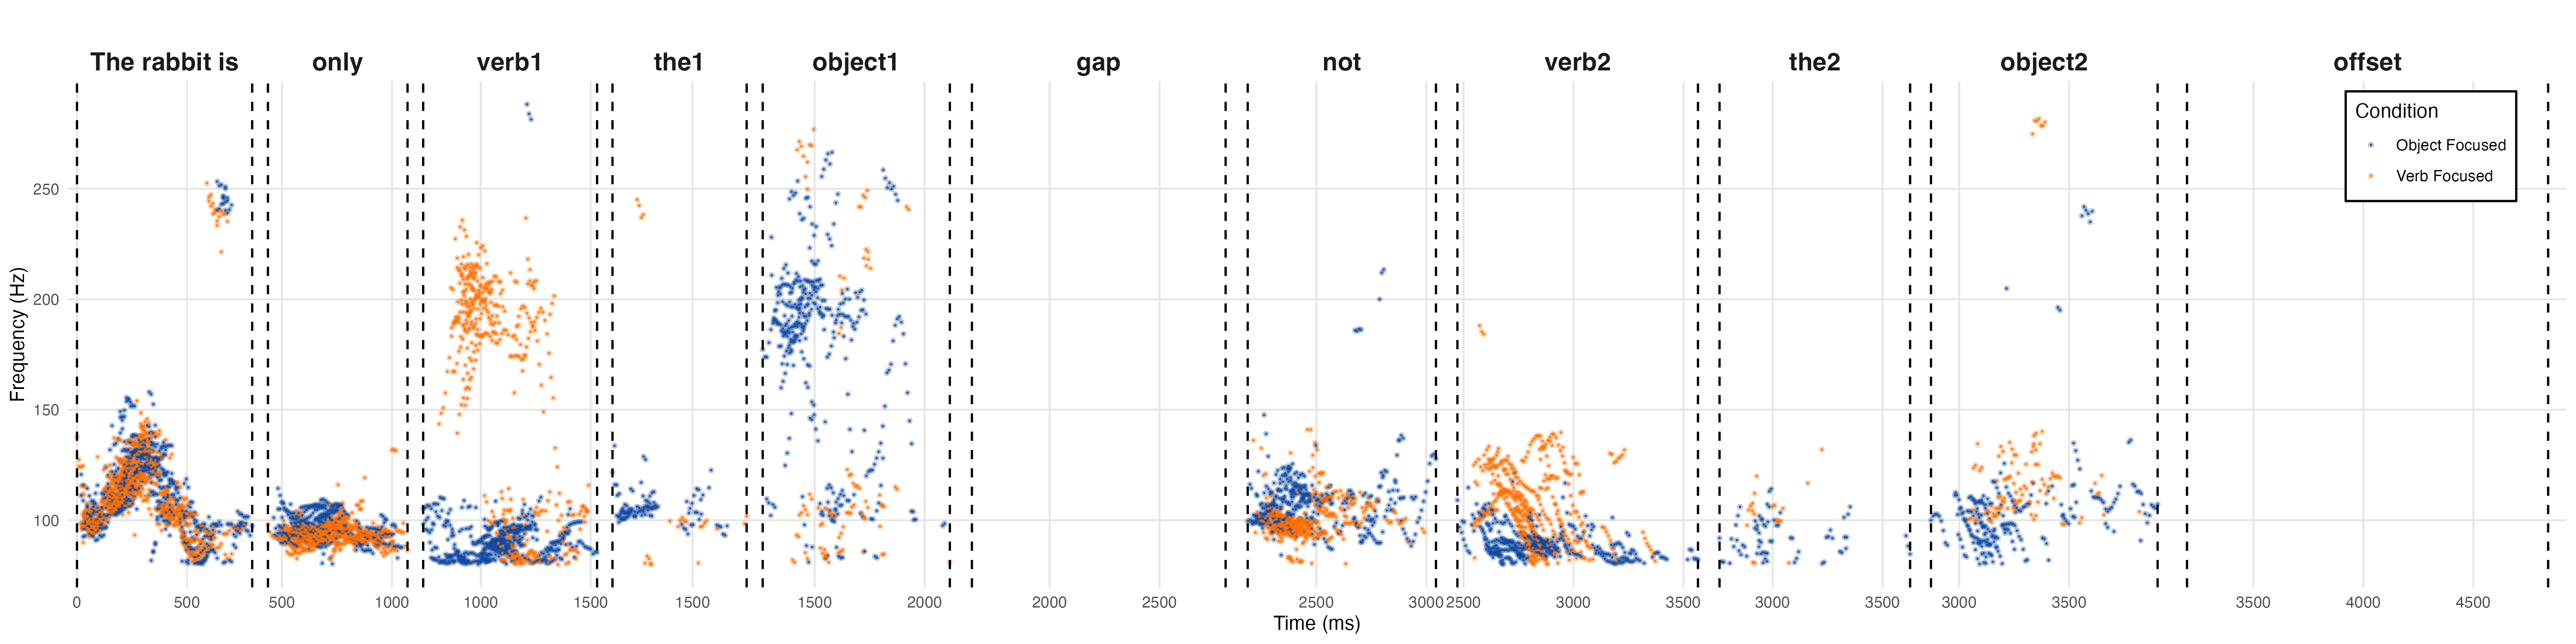
\includegraphics[width=\textwidth,height=\textheight,keepaspectratio]{viz/accoustic.png}
    \caption{Fundamental frequency over time by object-focused (blue) and verb-focused (orange) sentences.}
    \label{fig:acoustic}
\end{figure}

Figure \ref{fig:acoustic} highlights two key points. First, for verb-focused sentences (indicated in orange), we see an increase in F0 at the ``verb1" time bin and for object-focused sentences (indicated in blue), we see an increase in F0 at the ``object1" time bin. This figure suggests systematic variation in the way F0 information conveys focus. Second, F0 information is dynamic and unfolds over time. It is not the case that for every stimulus within the verb-focused condition that F0 cues increase the same amount or at the same time during the ``verb1" utterance. Here we ask whether this acoustic information contributes to the observed eye movements.

\subsection{Individuals differ in their language processing behavior}
%We know that individuals differ in nearly every linguistic measure. There are a finite number of variables that researchers can measure, and these measurements have informed our understanding of the mechanisms involved in language acquisition and processing \citep{Kidd2018, skehan1991individual, nelson1981individual}. 

Current experimental evidence suggests that there is a complex interplay between cognitive abilities, auditory perceptual abilities, and motor reproduction abilities during speech processing \citep{saito2022does, bramlett_wiener_24_speechprosody, bakkouche2025effects, Kachlicka_Saito_Tierney_2019}. Whereas we cannot review (and explore) every possible individual difference predictor, we briefly review the following five ways in which individuals differ as it relates to spoken language processing: working memory, cognitive control, lexical proficiency, auditory perception abilities, and auditory motor reproduction abilities.


\subsubsection{Working memory}
Working memory, or the ability to keep recent input in mind and later draw on it \citep[see][]{baddeley2003working,carpenter2013role} can affect a wide range of linguistic processes. How working memory affects the processing of focus prosody is unclear. To the best of our knowledge, this specific research question has not been asked. Based on findings related to working memory and prosody processing research \citep[e.g.,][]{traxler2009hierarchical,ferreira2015prosody, bishop2021exploring}, the answer most likely depends on the population, task demands, and methods used. For example, working memory, as measured by the digit span task (the same task we use in the present study), was not predictive in terms of identifying English emotional prosody \citep{sinagra2022perception} or Italian lexical stress \citep{ppcc} in groups of L1 adults, presumably given the relatively simple task demands of identifying happy/sad prosody or a penultimate/antepenultimate stressed word. In the present study, however, we use longer sentences involving potential object or verb targets that may require listeners to store linguistic information and draw on it later (i.e., upon hearing the ``not" in the sentence a listener must recall the earlier input). We also test both L1 and L2 listeners. It is not clear whether the task demands will place a burden on the listener's working memory, hence the inclusion of working memory as an exploratory variable.


\subsubsection{Cognitive control}
Whereas there are several cognitive tasks used in the psycholinguistics literature \citep{ness2023state}, we were interested in a task that captures participants' ability to resolve conflict during processing. For this reason, we used the Flanker task \citep{eriksen1974effects} in which 
participants must focus their attention on congruent stimuli (e.g., $>>>>>$) while resisting attention on incongruent stimuli (e.g., $>><>>$). Congruency tasks such as Flanker have been found to predict behavior in many different linguistic tasks and populations, especially bilinguals who must suppress their L1 while processing their L2 \citep{blumenfeld2014cognitive,luk2011there} (though see also \cite{hedge2018reliability} for reliability concerns). Here, we ask whether better cognitive control as indexed by performance on the Flanker task results in earlier eye movements to the alternative focus object, i.e., ``L1-like" timing of looks. We are unaware of research on cognitive control and focus processing in an L2, thus the exploratory nature of this question.



\subsubsection{Lexical proficiency}
L1 and L2 speakers differ in their lexical proficiency, which has unsurprisingly been shown to contribute to differences in language processing \citep{Yap2012, zareva2005relationship}. Here, we are interested in whether increased English lexical proficiency, as measured by the LexTALE task \citep{lemhofer2012introducing}, leads to earlier looks for the L2 English participants. That is, does a greater L2 proficiency result in more "L1-like" timing of eye movements? Although this particular research question has not been asked about focus processing (that we are aware of), there is evidence that higher proficiency scores are correlated with the speed of activation of the target and the degree to which lexical competition is resolved \citep{sarrett2022within}. It is not clear whether the ``look-and-listen" nature of our task will yield similar results, thus our exploratory question.

 

\subsubsection{Perceptual auditory sensitivity}
Detecting prosodic cues requires a certain level of sensitivity to incoming acoustics. English and Dutch both use F0 range expansion (or what listeners perceive as pitch), amplitude changes (intensity rise-time), and duration increases to convey focus. A growing body of research has explored auditory processing in L2 speech learning. Here we look at four measures of what \cite{saito2023does} calls ``explicit acuity in L2 speech learning:" how sensitive a listener is to temporal and spectral cues or dimensions (e.g., formant,
pitch, duration, and intensity). These measures have proven to be reliable measures for a range of L2 speech learning tasks \citep{Kachlicka_Saito_Tierney_2019, saito2024auditory, bakkouche2025effects, bramlett_wiener_24_speechprosody}. Here we extend this work to test whether these abilities are predictive of focus processing in \textit{only}-sentences. Once again, we are unaware of any previous research that has attempted to use these measures to predict L1 or L2 focus processing---though \cite{jansen2023influence} did show that musical perception ability, which aligns closely with our pitch task, was somewhat predictive of eye fixations. We further explore this area in our study.


\subsubsection{Auditory motor reproduction}
Finally, we explore whether auditory motor reproductions predict eye movements during focus processing. Here, we build on previous research that has argued for motor systems underlying both speech perception and production (e.g., \cite{liberman1985motor,hickok2011sensorimotor}). We examine whether participants' ability to reproduce target sound sequences for melodies (pitch) and rhythm (duration) is informative for understanding L1 and L2 prosodic processing. Recent work \citep{tierney2014auditory, saito2024auditory,tierney2017individual} has argued that motoric abilities are a crucial part of auditory processing and that the ability to integrate auditory input to motor actions helps explain various aspects of adult L2 acquisition. We are unaware of any work that has explored whether auditory motor reproduction abilities predict L1 or L2 focus processing, and therefore explore this predictor.

\subsection{Predictions guiding our exploratory analysis} 
We test whether the acoustic cues of F0, amplitude, duration, and spectral tilt predict eye movements. If there is an effect, we expect F0 and duration to be predictive of looks to the target/competitor. These cues may also interact with participants' perceptual abilities such that participants with better (or worse) pitch perception may behave differently given the acoustics. We also test whether participants with greater working memory look to the alternative focus object at an earlier point in time than those with reduced working memory. If there is an effect of working memory, we assume it will be found among all participants and not just within the L1 or L2 group. We also test whether participants with greater cognitive control (as measured by Flanker accuracy and response time) look to the alternative focus object at an earlier point in time than those with reduced cognitive control. If there is an effect of cognitive control, we assume it will be found among only the L2 participants and not the L1 group given the L2 group must suppress their L1 while performing the task. We also test whether participants with greater English lexical proficiency (as measured by LexTALE) look to the alternative focus object at an earlier point in time than those with reduced English lexical proficiency. If there is an effect of lexical proficiency, we assume it will be found among only the L2 participants and not the L1 group given the L1 group should have less variation in their English proficiency. We also test whether participants with greater perceptual auditory sensitivity look to the alternative focus object at an earlier point in time than those with reduced sensitivity. If there is an effect of auditory sensitivity, we assume it will be found among all participants given that the temporal and spectral cues or dimensions that we test---formant, pitch, duration, and intensity---are used in both Dutch and English for focus realization. Finally, we test whether participants with more accurate auditory motor reproductions look to the alternative focus object at an earlier point in time than those with less accurate reproductions. If there is an effect of motor reproductions, we assume it will be found among all participants given that this integration ability is necessary for all languages and underlies L1 and L2 speech perception.
